\section{Arkadiusz Baran}
TEST \emph{TEST} \underline{TEST} 
\section*{Przykładowe Wyrażenie Matematyczne}
Poniżej znajduje się wyrażenie opisujące wzór na pole powierzchni koła:

\begin{equation}
P = \pi r^2
\end{equation}

gdzie \( "P" \) to pole powierzchni, a \( "r" \) to promień.

\section*{Obrazek}

\noindent 
\\Tak Wygląda ananas (patrz Figure~\ref{fig:ananas})

\begin{figure}[htbp]
    \centering 
    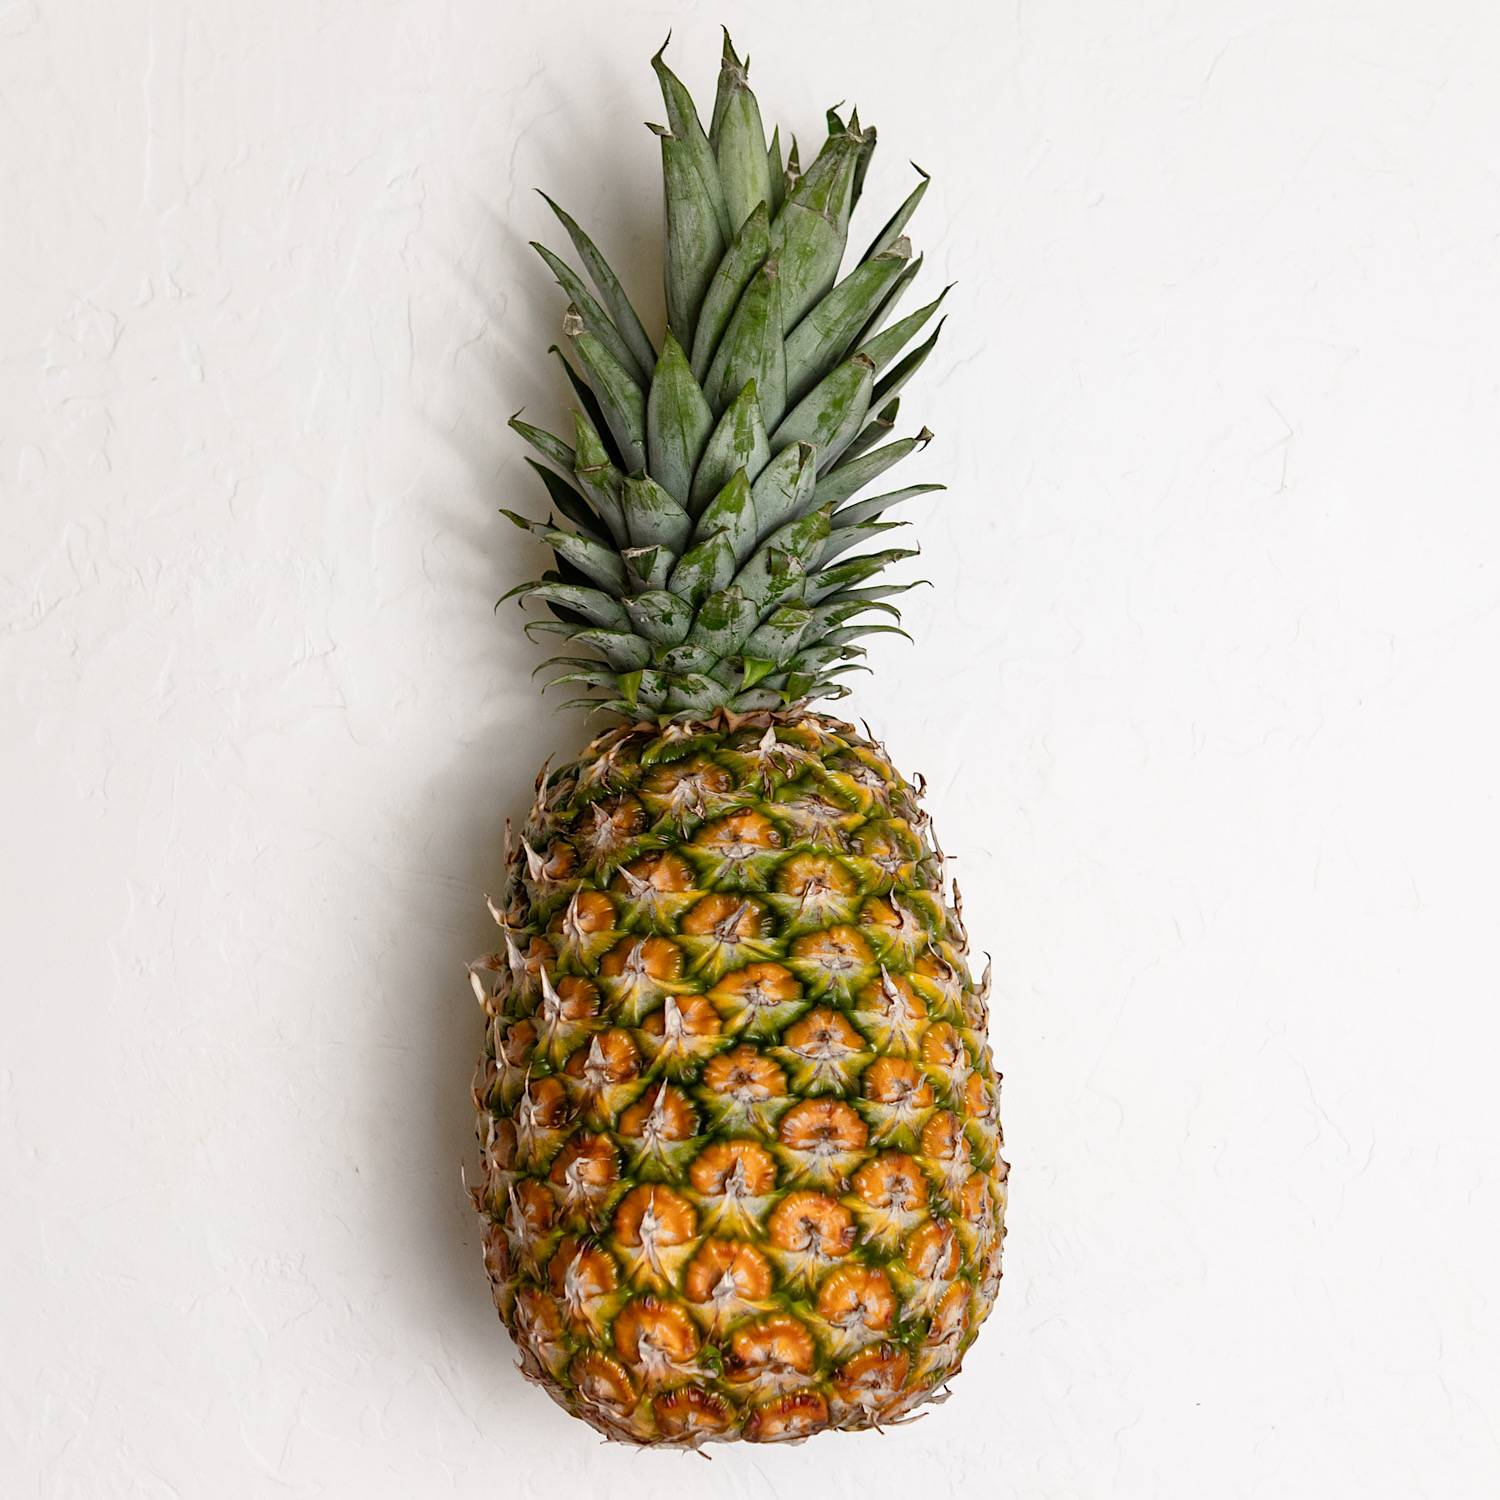
\includegraphics[width=0.5\linewidth]{pictures/ananas.jpg}
    \caption{Ananas Ananas}
    \label{fig:ananas}
\end{figure}

\noindent

\section*{Tabela}

Tabela \ref{tab:ananasszynka} przedstawia losowe słowa 

\begin{table}[hbtp]
\begin{tabular}{|
>{\columncolor[HTML]{FFCCC9}}c |
>{\columncolor[HTML]{FFCE93}}l |
>{\columncolor[HTML]{FFCCC9}}l |}
\hline
ananas & szczypta & {\color[HTML]{333333} ale} \\ \hline
\cellcolor[HTML]{FFCE93}szynka & \cellcolor[HTML]{FFCCC9}{\color[HTML]{000000} róży} & \cellcolor[HTML]{FFCE93}ucztta \\ \hline
mozzarella & wow & jej \\ \hline
\end{tabular}
\caption{TABELAAA TESTOWA }
\label{tab:ananasszynka}
\end{table}

\section*{Listy}
\noindent
\\Przykładowa lista numerowana:

\begin{enumerate}
    \item Pierwszy element.
    \item Drugi element.
    \item Trzeci element.
\end{enumerate}

\noindent
\\Przykładowa lista nienumerowana ze zmienionymi markerami:

\begin{itemize}
    \item[(*)] Pierwszy element.
    \item[(*)] Drugi element.
    \item[(*)] Trzeci element.
\end{itemize}


\section*{Przykładowy tekst z formatowaniem}
\textbf{Lorem ipsum dolor sit amet, consectetur adipiscing elit. Nunc viverra turpis sed lobortis vulputate.} Pellentesque auctor a dolor quis condimentum neque a egestas. 

\underline{Sed sodales lectus purus, quis maximus nulla commodo sed.} Morbi pellentesque tempor auctor. Suspendisse eu tellus diam. Curabitur molestie arcu nulla, sit amet varius diam fringilla sed. 

\emph{Nullam luctus sapien quis nibh varius, nec tempor ante tristique. Proin non risus est. Etiam a congue elit.} Integer ullamcorper efficitur lectus sit amet condimentum. Morbi gravida ornare massa nec dapibus.